\documentclass[12pt]{article}
\usepackage{hyperref}
\usepackage{graphicx}

\begin{document}
\begin{titlepage}
\newcommand{\HRule}{\rule{\linewidth}{0.5mm}} % Defines a new command for the horizontal lines, change thickness here

\center % Center everything on the page
%----------------------------------------------------------------------------------------
%	HEADING SECTIONS
%----------------------------------------------------------------------------------------
\textsc{\LARGE Swinburne University}\\[1.5cm] % Name of your university/college

%----------------------------------------------------------------------------------------
%	TITLE SECTION
%----------------------------------------------------------------------------------------
\HRule \\[0.4cm]
{ \huge \bfseries Cave Escape Presentation Guide}\\[0.4cm] % Title of your document
\HRule \\[1.5cm]

%----------------------------------------------------------------------------------------
%	AUTHOR SECTION
%----------------------------------------------------------------------------------------
\Large \emph{Authors:}\\
Jake \textsc{Renzella} and Reuben \textsc{Wilson}\\[1cm] % Your name

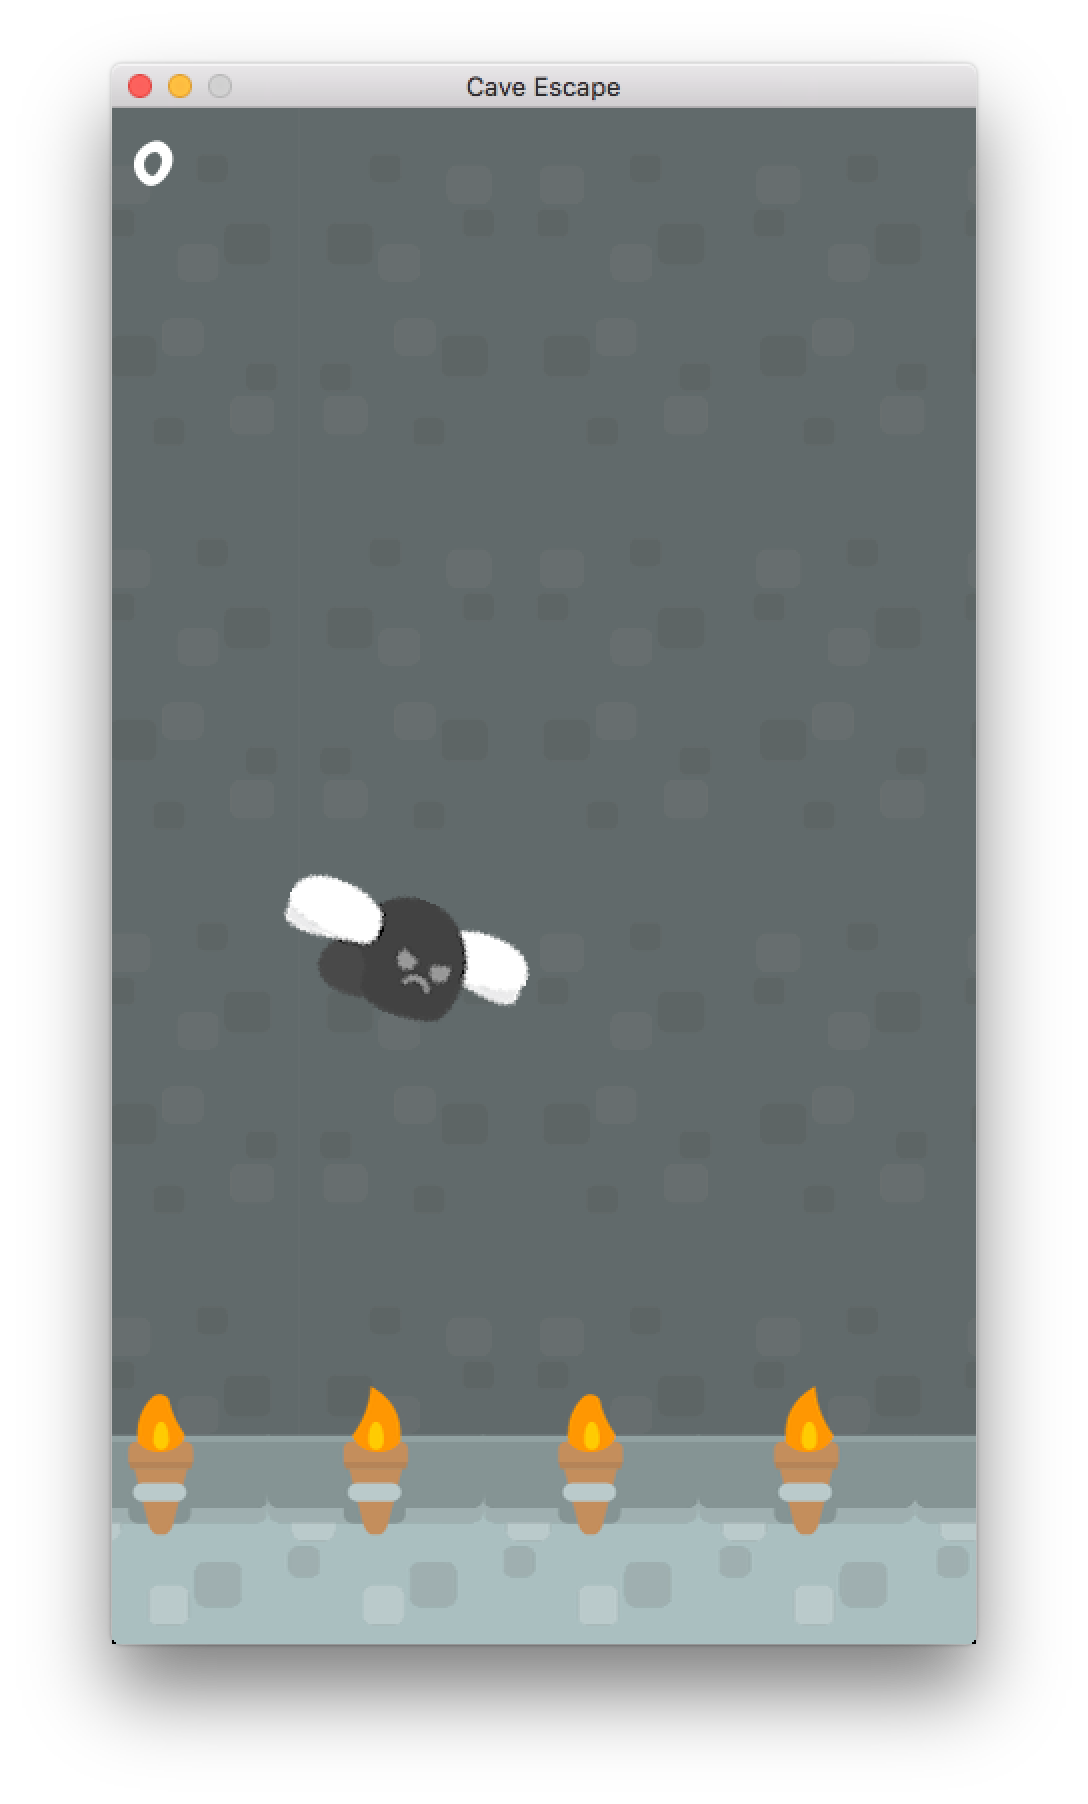
\includegraphics[scale=0.12]{FinalGame}\\

%----------------------------------------------------------------------------------------
%	DATE SECTION
%----------------------------------------------------------------------------------------
{\large \today}\\[3cm] % Date, change the \today to a set date if you want to be precise

%----------------------------------------------------------------------------------------
%	LOGO SECTION
%----------------------------------------------------------------------------------------
 % Include a department/university logo - this will require the graphicx package

%----------------------------------------------------------------------------------------

\vfill % Fill the rest of the page with whitespace

\end{titlepage}

\section{Introduction}
Cave Escape is a clone of the popular mobile game Flappy Bird which has been made in
Pascal using SwinGame. This presentation uses snapshots of the games progress as it was developed.
\newline
\newline
The aim of the presentation is to show the audience the basics of how game development works, just how simple making
a game can be, and how much fun they can have.
\newline
\newline
Throughout the course of the presentation, the Presenter will present different iterations of the code of the game, in different levels of completion and
talk about what each new addition to the code does to the program/game.
\newline
\newline
All versions of code shown to the auidience will be complete, meaning they are executable. The purpose is to allow the presenter to visualise
with the audience what different blocks of code actually do to the game.
\newline
\newline
The presenter should have enough procedural programming knowledge and experience to talk through all lines of the code, and answer any questions about the code.

\subsection{Installation}
The development envioronment of Swingame using Pascal requires a few tools to be isntalled that the presenter or audience
may not have. Thankfully, there are detailed instructions in the form of videos which run through installing the necessary tools to compile SwinGame.

The presenter will not need these tools to present, this package is precompiled and ready to go, however if the audience would like to alter the source code
for their own versions of the game, they should be directed to the videos on
\href{https://www.youtube.com/playlist?list=PLdVESrjTNUXtU8zclRh9ovhstzWQAY05U}{\underline{YouTube}} and chose the isntallation videos.
\pagebreak

\section{\Large\textbf{Presentation}}

\subsection*{File 1}
The first code file provided is a basic game loop in SwinGame. Running the application will open a graphics window, however it will not display anything (as nothing has been drawn to the window!).
At this stage the presenter should talk about how the lines of code are run in sequence.

\subsection*{File 2}
The second code file provided adds and draws a sprite of our player, the background, and the foreground to the screen, but not much else. Nothing is moving.
Talk about how we added the sprite's image to the resource bundle, and how we load the image in our code.

\subsection*{File 3}
The third code file provided adds the functionality which makes the player fall (gravity), but no user input is handled so the player just falls off the screen!
Talk about how this is a start, however is pretty boring still.

\subsection*{File 4}
The fourth code file provided allows the player to jump when the user presses a button. Talk about how this is achieved in the code.

\subsection*{File 5}
Version 5 of the code file adds in the poles bitmaps to the resources folder, and adds the code for their placement and drawing on the screen. It also
adds the code for moving them off the screen and resetting them. This is a big jump in code so spend some time talking about how we place them,how
we detect that they have moved off the screen, and how we reset them.
\newpage
\subsection*{File 6}
This version adds the code for collision detection between the player and the poles, and the player and the ground and sky. Talk about how we detect collisions, how we
reset the game when a collision is detected etc. Talk about how we basically have a complete game here, we have:

\begin{itemize}
\item A moving player
\item Scrolling poles
\item collision detection
\item physics
\end{itemize}

While we have a complete game, it can definitely be spruced up a bit.

\subsection*{File 7}
Version 7 is the final source code for Cave Escape. We have added animations, music, and a score to create a much more enjoyable and functional game.
Talk about how simple a game like this can be (only 250 or so lines of code).

\section*{Conclusion}
At this point, take any questions, ask the audience how we could possible modify the game, how we could create other games etc.

\end{document}
